\chapter{O Tema da Tese}

A tese obrigatoriamente tem que ter um assunto, que deve ser escolhido no início do trabalho. Essa escolha é importante e deve ser feita com cuidado, de modo a que permita ao candidato crescer academicamente, contribuir para o conhecimento e, ao mesmo tempo, evitar dissabores.

\gxatencao{O aluno deve se identificar com o tema de tese escolhido.}

Você não vai conseguir acabar uma tese da qual não goste do tema desde o início do seu trabalho. Mesmo gostando do tema inicialmente, é possível que no fim da tese você não queira ver mais o tema “nem pintado”, o que não é bom, mas pelo menos você terminou a tese.

O tema deve ser escolhido com muito cuidado. Primeiro, deve ser de seu interesse, praticamente uma paixão. Segundo, deve ser de interesse do orientador. Finalmente deve ser do interesse da comunidade científica.

Alguns temas, mesmo sendo de interesse pessoal, não interessam a ninguém.

Ou por já estarem resolvidos, ou por não serem ainda percebidos, ou pior, porque não têm valor científico, ou não têm valor na comunidade científica a que o candidato pertence.

Normalmente se faz um plano de tese no início. Esse plano nem sempre é seguido, pois com o tempo entendemos melhor o problema, suas formas mais genéricas ou mais específicas, e alterações de rota são feitas.

Não se preocupe muito no início, no primeiro ano do doutorado, ou nos três primeiros meses de pesquisa no mestrado, se seu tema é incerto. Seu objetivo deve ser fixado nesse prazo, mas o mais importante é entender o contexto do tema e os problemas importantes a serem resolvidos. Depois, nos próximos 2 ou 3 anos, você irá em direção a fechar a tese.

Para escolher o tema, é importante que você escolha cadeiras que tenham relação com assuntos de seu interesse. Não escolha cadeiras pela facilidade ou pelo horário disponível, escolha cadeiras que lhe ajudem a escolher e estudar temas de seu interesse.

% TODO: \usepackage{graphicx} required
\begin{figure}[hbt]
    \centering
    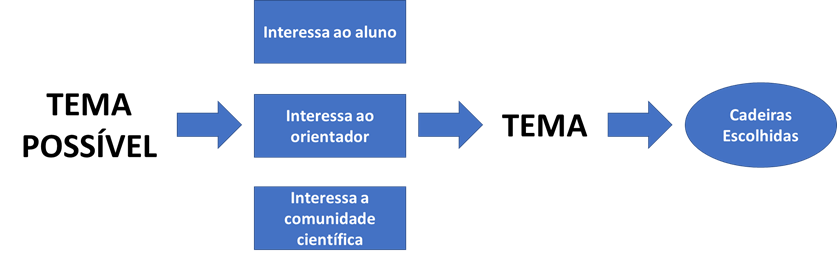
\includegraphics[width=0.9\linewidth]{Images/escolhatemacadeiras}
    \caption{Escolhendo tema e cadeiras. Fonte: o autor}
    \label{fig:escolhatemacadeiras}
\end{figure}


\section{O que é uma Contribuição Original}

Um dos requisitos da tese de doutorado é possuir uma contribuição original.

Eu confesso que contribuição original não é uma definição muito clara. Vamos analisar, então, o que é uma contribuição.

A professora Marta Mattoso diz que :
\begin{itemize}
\item	“Uma contribuição é um resultado que pode ser útil para outras pessoas.”
\item	“O resultado é uma novidade e não poderia ser afirmado sem o desenvolvimento da tese.”
\end{itemize}

Ou seja, uma contribuição pode se algo como encontrado na lista a seguir, levemente ordenada da maior para a menor e de forma não exaustiva.
\begin{enumerate}
\item	A solução de um problema em aberto;
\item	Uma melhoria comprovada a alguma prática da área;
\item	A proposta de uma metodologia, método ou processo que resolva um problema do mundo real, com uma abordagem científica;
\item	Aplicar uma prática da área em uma área de aplicação, de maneira não trivial;
\item	A investigação de um problema que descobre novas evidências na área;
\item	A criação de sistemas complexos envolvendo várias práticas até antes isoladas, com um resultado científico palpável;
\item	A comparação e análise de diferentes soluções computacionais para o mesmo problema, com consequente desenvolvimento de solução que as agregam de alguma forma;
\item	O levantamento de uma história, ou o estudo de casos, que trazem contribuição original para o entendimento de como algo aconteceu ou acontece, sempre de acordo com metodologias reconhecidas;
\item	A criação de novas bases de dados que podem servir para outros trabalhos.
\end{enumerate}

Porém, ao contrário de outras áreas, no Programa de Engenharia de Sistemas e Computação, e em toda COPPE, não é considerada uma contribuição;
\begin{itemize}
    \item 	Fazer a compilação de dados ou informações já existentes (como a criação de um review da área);
    \item	Desenvolver aplicações convencionais com software disponível amplamente;
    \item 	Desenvolver protótipos com tecnologia amplamente conhecida e divulgada.

\end{itemize}

Veja que a tese tem que comprovar a contribuição. Não basta dizer que algo é bom e original, é importante poder provar que é melhor (mesmo que dentro de alguns casos) e que não há outro resultado igual, ou ainda que abre um caminho novo de pesquisa.

\section{Como encontrar uma Contribuição}

Normalmente em uma tese de computação existe um problema, uma solução e uma comprovação ou validação da solução.

Assim, uma tese pode apresentar contribuições nessas três áreas. Lidando com o problema, podemos encontrar novos problemas ainda não tratados e modelar de formas diferentes problemas já tratados.

Na solução, podemos aplicar técnicas já existentes em problemas ainda não tratados com elas ou inventar novas técnicas. Finalmente, podemos trabalhar arduamente nas técnicas de comprovação de nossos resultados, principalmente quando esses resultados são experimentais ou empíricos\footnote{Em soluções teóricas é necessário provar que a solução é verdadeira, porém isso normalmente é parte da própria solução. Porém, existem teses teóricas que apresentam novas formas, mais simples, de provar um teorema já provado}.

O importante é ter um problema bem claro. Esse problema pode já ter sido proposto antes, ou pode ser levantado. Uma maneira de levantar problemas é estudar soluções já existentes e ver quando elas falham, ou que lacunas elas têm.

Listar as falhas ou lacunas de uma situação atual é um bom método de descobrir onde você pode trabalhar. As lacunas podem ser elencadas, algumas podem ser selecionadas, e toda a tese construída em torno desse conceito.

Muitos alunos querem começar pela solução, algo do tipo “quero usar a técnica X”. Esse não é um bom caminho, apesar de já ter funcionado para algumas pessoas. Porém, o que acontece normalmente é que o aluno fica com uma solução a procura de um problema e não tem como comprovar a qualidade ou a utilidade de sua solução.


\section{Pensando sua Tese}

Várias técnicas podem ser usadas para você pensar sua tese.

Algumas técnicas são muito úteis. Uma delas é a \gxdefine{5W2H}, responder as perguntas: Why, What, Who, When, Where, How e How Much. Essa é das técnicas mais gerais e mais úteis. Principalmente se perguntar “Por que estou fazendo isso” e “Quem vai ser beneficiado” permitem justificar plenamente o trabalho de sua tese, fazendo com que ela não fique perdida em um contexto vago.  A Figura \ref{fig:5w2h} mostra algumas perguntas possíveis nessa técnica.

% TODO: \usepackage{graphicx} required
\begin{figure}[hbt]
    \centering
    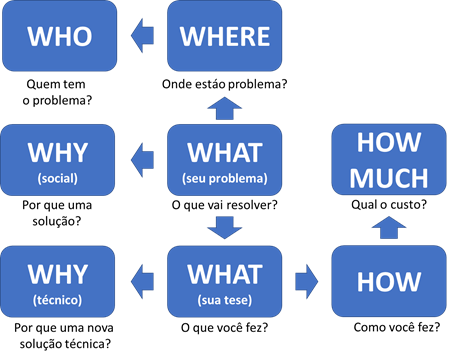
\includegraphics[width=0.7\linewidth]{Images/5w2h}
    \caption{Perguntas que devem ser respondidas antes de iniciar uma tese. Fonte: do autor.}
    \label{fig:5w2h}
\end{figure}




Algumas teses atuais têm proposto lacunas no estado da arte, e a partir dessas lacunas geram questões de pesquisa, que por sua vez podem gerar objetivos gerais e específicos. Esse é outro bom quadro teórico para trabalhar.

Entre meus alunos, o uso da \gxdefine{Design Science Research} (\gxdefine{DSR})\citep{Pimentel2020} também fornece caminhos para pensar sua tese . Eu estou me tornando cada vez mais um adepto dessa metodologia, dessa forma de fazer Ciência, que é realizada por meio de vários processos mais detalhados. Ou seja, não existe um método científico DSR, ele é mais uma filosofia de trabalho que fornece parâmetros para estabelecer um método específico.

Outra técnica possível, é desenhar um \gxdefine{Project Model Canvas}\footnote{\url{http://www.projectmodelcanvas.com/}} . Essa é uma proposta de José Finocchio Júnior e tem uma representação visual interessante, apresentada na Figura \ref{fig:pmc}.

% TODO: \usepackage{graphicx} required
\begin{figure}
    \centering
    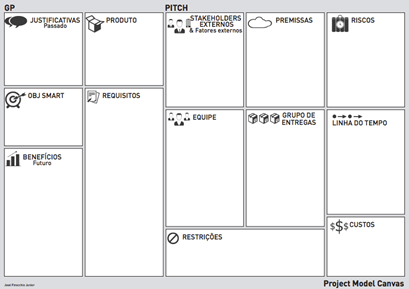
\includegraphics[width=0.7\linewidth]{Images/PMC}
    \caption{Representação do Project Model Canvas de José Finocchio Júnior (CC:BYNOND)}
    \label{fig:pmc}
\end{figure}


\section{Como descrever o que é a tese}

Algumas coisas são importantes para você definir sua tese.

Primeiro, você tem que \textbf{conhecer um problema} e o \textbf{estado da arte da solução} do problema. Se seu orientador trabalha com o problema, você ainda tem que conhecer bem o trabalho que ele tem feito, para entrar realmente no grupo.

Segundo, é interessante que você consiga dar um \textbf{valor} a esse problema\footnote{Você pode ouvir uma aula sobre valor em \url{https://youtu.be/aOQQHGzC-YE}, ou ler o capítulo sobre valor escrito em \url{https://github.com/xexeo/MaterialEducacional}} . O valor pode ser econômico, como a diminuição de um custo, pode ser um valor acadêmico, como um teorema em aberto a muito tempo, ou pode ser outra forma de valor, como social ou histórico. Uma visão rápida de Valor, típica da Engenharia de Software, é procurar 3 coisas: aumentar o faturamento (benefícios), reduzir custos e melhorar serviços.

Terceiro, você deve ter uma \textbf{proposta de abordagem ao problema}. Isto significa que você deve entender caminhos possíveis para resolvê-lo e ter uma ideia das técnicas que pretende adotar.

Todas essas coisas podem ser descritas de várias formas, tanto ao longo do trabalho em apresentações como no texto final. Algumas abordagens mais tradicionais que outras.

\section{A descrição da tese na introdução}

Na introdução da sua tese deve existir uma descrição do que ela é e que deixe o leitor totalmente ciente do que vai encontrar durante a leitura.

Por exemplo, é importante \textbf{definir o problema} que a tese trata. Esse problema deve ocorrer dentro de um \textbf{contexto}. Também deve ficar claro o \textbf{objetivo} da tese. Esse objetivo pode ser dividido em \textbf{questões de pesquisa}, que devem levar gradativamente ao objetivo, ou pode gerar \textbf{conjecturas} que precisam ser comprovadas ou pelo menos validadas, já que certas conjecturas são difíceis de serem comprovadas de forma absoluta, devido a incluírem, por exemplo, aspectos do comportamento humano.

Costumamos, reservar o termo \textbf{hipótese para conjecturas que podem ser provadas com experimentos} que incluem uma hipótese nula, por meios estatísticos, ou provada, ou negada, por meio de um teorema. Chamar de hipótese, no corpo da tese, algo que não pode ser comprovado dessa forma, cria uma expectativa errada no leitor. Caso não haja uma comprovação formal, devemos evitar o termo hipótese e usar outros como conjecturas ou questões de pesquisa.

Podem ser necessárias também a elaboração de uma ou mais \textbf{premissas}, que são afirmações consideradas válidas a priori para sua tese. Premissas não são questionadas ao logo da tese, e sim assumidas como válidas. Claro que se espera que as premissas tenham alguma evidência, ou seja, não sejam facilmente falseáveis.

\section{A Metodologia DSR Adotada por Mim}

Design Science Research (DSR) é uma abordagem metodológica que visa a construção e avaliação de artefatos para resolver problemas complexos no contexto das ciências aplicadas, como a Engenharia de Software, Sistemas de Informação e Ciência da Computação em geral~\citep{hevner2004design}. 

A DSR diferencia-se das abordagens tradicionais por focar não apenas na compreensão do fenômeno, mas na intervenção com base em um conhecimento científico rigoroso \cite{hevner2004design, peffers2007design}. Assim, ela busca contribuir tanto para a prática quanto para a teoria.

A orientação atual ao adotar a DSR é modelar o trabalho com o método MODEL-DSR~\citep{pimentel2019dsr,pimentel2023} e produzir os artefatos segundo o \textit{Framework de Pesquisa em Tecnologia da Informação}~\citep{march1995design}.


\subsection{Um Modelo de Pesquias em DSR - MODEL-DSR}

O MODEL-DSR é uma proposta metodológica desenvolvida por Pimentel, Filippo e Santoro \cite{pimentel2019dsr,pimentel2023}, com o objetivo de orientar pesquisas em Informática na Educação a partir dos princípios da Design Science Research. 

Segundo \citet{pimentel2023} ``O modelo consiste em um conjunto de elementos que precisam estar coerentemente inter-relacionados''. Dado um problema que existe dentro de um contexto, um artefato é construído direcionadas por conjecturas comportamentais. O artefato então permite a avaliação do problema em contexto e da conjectura (ver \autoref{fig:dsrmodel})

\begin{figure}
    \centering
    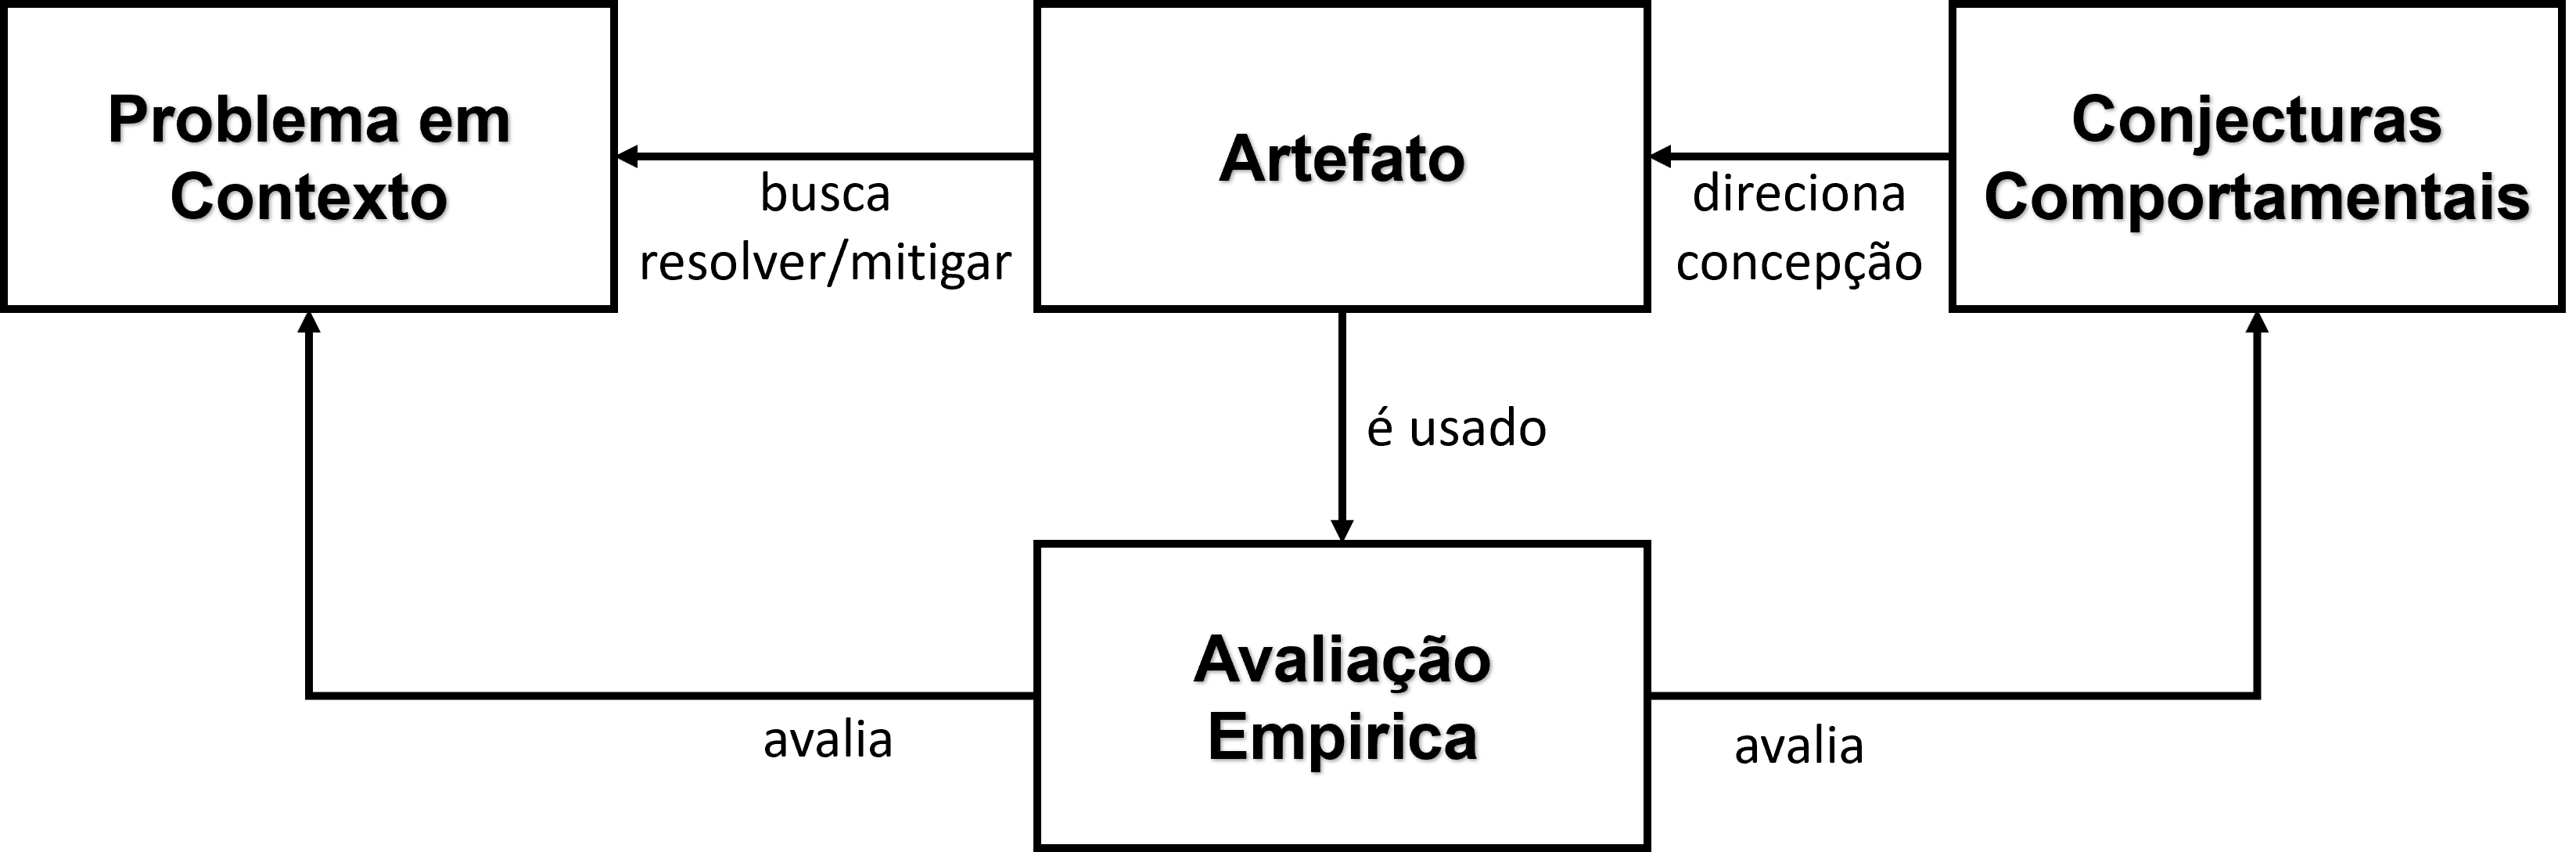
\includegraphics[width=0.5\linewidth]{Images/dsr pimental.png}
    \caption{Elementos centrais do Model-DSR. Baseado em \citep{pimentel2023}}
    \label{fig:dsrmodel}
\end{figure}

O modelo também propõe um artefato visual que explicita as conexões entre teoria, problema, solução e contexto. Esse artefato é adotado por nosso grupo para definir a pesquisa que está sendo feita. Exemplos foram dados por \citet{pimentel2019dsr} e \citet{pimentel2023}.

Ao destacar a produção de conhecimento científico como elemento central da DSR, o MODEL-DSR contribui para diferenciar claramente pesquisa de desenvolvimento tecnológico. Ele é especialmente adequado a pesquisas aplicadas em educação mediada por tecnologia, promovendo o rigor metodológico e a relevância prática.

\subsection{Framework de Pesquisa em Tecnologia da Informação}

March e Smith \cite{march1995design} propuseram um framework bidimensional (ver \autoref{tab:marchsmith}) para pesquisas em Tecnologia da Informação que distingue entre tipos de artefatos produzidos e atividades de pesquisa realizadas. Os artefatos incluem:
\begin{itemize}
    \item \textbf{Construtos}: são os conceitos que formam a linguagem da área de estudo, usados para descrever problemas e formular soluções.
    \item \textbf{Modelos}: expressam relações entre construtos e servem como representacões de situações-problema ou de soluções.
    \item \textbf{Métodos}: são sequências de passos ou algoritmos utilizados para resolver tarefas específicas.
    \item \textbf{Instâncias}: são realizações concretas de sistemas, ferramentas ou protótipos que demonstram o uso prático dos construtos, modelos e métodos.
\end{itemize}

As atividades de pesquisa compreendem:
\begin{itemize}
    \item \textbf{Construção (build)}: desenvolvimento dos artefatos para um objetivo específico, demonstrando sua viabilidade.
    \item \textbf{Avaliação (evaluate)}: análise sistemática do desempenho dos artefatos em função de métricas e critérios estabelecidos.
    \item \textbf{Teorização (theorize)}: construção de explicações que descrevem como e por que os artefatos funcionam em seu ambiente.
    \item \textbf{Justificativa (justify)}: verificação empírica ou formal das teorias propostas, com base em evidências.
\end{itemize}

Esse framework contribui para organizar e avaliar as pesquisas em TI segundo seu tipo de contribuição, facilitando a compreensão e a comunicação dos resultados científicos.





\begin{table}[hbt]
    \centering
    \begin{tabular}{|c|c|c|c|c|}
    \hline
       & Construção & Avaliação & Teorização & Justificativa  \\    \hline
    Construtos &&&&\\     \hline
    Modelo &&&&\\    \hline
    Método &&&&\\    \hline
    Instâncias &&&&\\    \hline
    \end{tabular}
    \caption{O \textit{Framework} de pesquisa em tecnologia da informação proposto por \citet{march1995design}}
    \label{tab:marchsmith}
\end{table}

Além disso, Hevner et al. \cite{hevner2004design} destacam que a contribuição para o corpo de conhecimento científico é um critério essencial para a validade de uma pesquisa baseada em DSR.

